\documentclass[a4paper,openright,9pt]{report}
\usepackage[utf8]{inputenc}
\usepackage[a4paper]{geometry}
\geometry{top=2cm, bottom=2cm, left=1.5cm, right=1.5cm}
\usepackage{graphicx}
\usepackage{booktabs}
\usepackage{wrapfig}
\usepackage[rightcaption]{sidecap}
\usepackage{float}
\usepackage{tabulary}
\usepackage{array}
\usepackage{multirow,array}
\usepackage{listings}
\usepackage{hyperref}
\usepackage{color} %red, green, blue, yellow, cyan, magenta, black, white
\usepackage{hyperref}
\usepackage{setspace}
\usepackage{caption}
\usepackage{subcaption}
\usepackage{placeins}
\usepackage[arrowmos]{circuitikz}
%otro paquete para circuitos que me parece mas facil
\usepackage{tikz}
\usepackage{fancybox}
\usepackage{array}
\usepackage{remreset}
\usepackage{titlesec}
\renewcommand{\thesection}{\arabic{section}}
\usepackage{comment}
\usepackage{siunitx}
\setcounter{secnumdepth}{4} %Para poner sub subsecciones (\subsubsection{<subsection>}) y para un nivel mas de subsección hay que poner \paragraph{<subsubsubsection>}
\titlelabel{\thetitle.\quad} %Para que ponga un punto desdpues de numerar una sección
\usepackage{mathtools}
\DeclarePairedDelimiter{\abs}{\lvert}{\rvert} %definir modulo como \abs{}
\usepackage{physics} %Este paquete tiene derivadas mas chetas:
%	\dv{Q}{t} = \dv{s}{t}		 	para derivadas comun
%	\dv[n]{Q}{t} = \dv[n]{s}{t} 	para derivadas comun sucesivas (segunda derivada, tercera, etc..)
%
%	\pdv{Q}{t} = \pdv{s}{t}  		para derivadas parciales
%	\pdv[n]{Q}{t} = \pdv[n]{s}{t}
%	\pdv{Q}{x}{t} = \pdv{s}{x}{t} 	para derivadas parciales multiples distintas
\newcommand{\code}[1]{\texttt{#1}} %Para escribir texto como codigo \code{<codigo>}

\renewcommand{\tablename}{Tabla} %Para que diga "Figura" en vez de "Figure"


\ctikzset{bipoles/voltmeter/text rotate/.initial=0,% <=new key
rotationvolt/.style={bipoles/voltmeter/text rotate=#1},% style for ease introduction in code
}

% code from pgfcircbipoles.sty
\makeatletter
\pgfcircdeclarebipole{}{\ctikzvalof{bipoles/voltmeter/height}}{voltmeter}{\ctikzvalof{bipoles/voltmeter/height}}{\ctikzvalof{bipoles/voltmeter/width}}{
    \def\pgf@circ@temp{right}
    \ifx\tikz@res@label@pos\pgf@circ@temp
        \pgf@circ@res@step=-1.2\pgf@circ@res@up
    \else
        \def\pgf@circ@temp{below}
        \ifx\tikz@res@label@pos\pgf@circ@temp
            \pgf@circ@res@step=-1.2\pgf@circ@res@up
        \else
            \pgf@circ@res@step=1.2\pgf@circ@res@up
        \fi
    \fi

    \pgfpathmoveto{\pgfpoint{\pgf@circ@res@left}{\pgf@circ@res@zero}}
    \pgfpointorigin \pgf@circ@res@other =  \pgf@x  \advance \pgf@circ@res@other by -\pgf@circ@res@up
    \pgfpathlineto{\pgfpoint{\pgf@circ@res@other}{\pgf@circ@res@zero}}
    \pgfusepath{draw}

    \pgfsetlinewidth{\pgfkeysvalueof{/tikz/circuitikz/bipoles/thickness}\pgfstartlinewidth}

        \pgfscope
            \pgfpathcircle{\pgfpointorigin}{.9\pgf@circ@res@up}
            \pgfusepath{draw}
        \endpgfscope

    \pgftransformrotate{\ctikzvalof{bipoles/voltmeter/text rotate}}% <= magic line
    \pgfsetlinewidth{\pgfstartlinewidth}

    \pgfsetarrowsend{latex}
    \pgfpathmoveto{\pgfpoint{\pgf@circ@res@other}{\pgf@circ@res@down}}
    \pgfpathlineto{\pgfpoint{-\pgf@circ@res@other}{\pgf@circ@res@up}}
    \pgfusepath{draw}
    \pgfsetarrowsend{}

    \pgfpathmoveto{\pgfpoint{-\pgf@circ@res@other}{\pgf@circ@res@zero}}
    \pgfpathlineto{\pgfpoint{\pgf@circ@res@right}{\pgf@circ@res@zero}}
    \pgfusepath{draw}


    \pgfnode{circle}{center}{\textbf{V}}{}{}
}

\makeatother

\ctikzset{bipoles/ammeter/text rotate/.initial=0,% <=new key
rotationamper/.style={bipoles/ammeter/text rotate=#1},% style for ease introduction in code
}

\makeatletter
\pgfcircdeclarebipole{}{\ctikzvalof{bipoles/ammeter/height}}{ammeter}{\ctikzvalof{bipoles/ammeter/height}}{\ctikzvalof{bipoles/ammeter/width}}{
    \def\pgf@circ@temp{right}
    \ifx\tikz@res@label@pos\pgf@circ@temp
        \pgf@circ@res@step=-1.2\pgf@circ@res@up
    \else
        \def\pgf@circ@temp{below}
        \ifx\tikz@res@label@pos\pgf@circ@temp
            \pgf@circ@res@step=-1.2\pgf@circ@res@up
        \else
            \pgf@circ@res@step=1.2\pgf@circ@res@up
        \fi
    \fi

    \pgfpathmoveto{\pgfpoint{\pgf@circ@res@left}{\pgf@circ@res@zero}}
    \pgfpointorigin \pgf@circ@res@other =  \pgf@x  \advance \pgf@circ@res@other by -\pgf@circ@res@up
    \pgfpathlineto{\pgfpoint{\pgf@circ@res@other}{\pgf@circ@res@zero}}
    \pgfusepath{draw}

    \pgfsetlinewidth{\pgfkeysvalueof{/tikz/circuitikz/bipoles/thickness}\pgfstartlinewidth}

        \pgfscope
            \pgfpathcircle{\pgfpointorigin}{.9\pgf@circ@res@up}
            \pgfusepath{draw}
        \endpgfscope

    \pgftransformrotate{\ctikzvalof{bipoles/ammeter/text rotate}}% <= magic line
    \pgfsetlinewidth{\pgfstartlinewidth}

    \pgfsetarrowsend{latex}
    \pgfpathmoveto{\pgfpoint{\pgf@circ@res@other}{\pgf@circ@res@down}}
    \pgfpathlineto{\pgfpoint{-\pgf@circ@res@other}{\pgf@circ@res@up}}
    \pgfusepath{draw}
    \pgfsetarrowsend{}

    \pgfpathmoveto{\pgfpoint{-\pgf@circ@res@other}{\pgf@circ@res@zero}}
    \pgfpathlineto{\pgfpoint{\pgf@circ@res@right}{\pgf@circ@res@zero}}
    \pgfusepath{draw}


    \pgfnode{circle}{center}{\textbf{A}}{}{}
}
\makeatother

\usepackage{etoolbox,refcount}
\usepackage{multicol}

\newcounter{countitems}
\newcounter{nextitemizecount}
\newcommand{\setupcountitems}{%
  \stepcounter{nextitemizecount}%
  \setcounter{countitems}{0}%
  \preto\item{\stepcounter{countitems}}%
}
\makeatletter
\newcommand{\computecountitems}{%
  \edef\@currentlabel{\number\c@countitems}%
  \label{countitems@\number\numexpr\value{nextitemizecount}-1\relax}%
}
\newcommand{\nextitemizecount}{%
  \getrefnumber{countitems@\number\c@nextitemizecount}%
}
\newcommand{\previtemizecount}{%
  \getrefnumber{countitems@\number\numexpr\value{nextitemizecount}-1\relax}%
}
\makeatother
\newenvironment{AutoMultiColItemize}{%
\ifnumcomp{\nextitemizecount}{>}{3}{\begin{multicols}{2}}{}%
\setupcountitems\begin{itemize}}%
{\end{itemize}%
\unskip\computecountitems\ifnumcomp{\previtemizecount}{>}{3}{\end{multicols}}{}}

\begin{document}

\vspace{\fill}
% Logo FIUBA - imagen no incluida en este documento

\begin{center}

\Huge{Trabajo Practico Control Adaptativo}
\\
\Huge{Identificación Paramétrica Exitosa: Modelo ARMAX}
\bigskip \\
\small{Gaggino, Lucas - Padrón: 99110}
\\

\small{\textit{86.20 Control Adaptativo }}
\\
\small{\textit{Departamento de Electrónica, Facultad de Ingeniería, UBA}}\\
\indent

\end{center}
\vspace{\fill}
\newpage

\section{Introducción}

Este trabajo práctico demuestra el \textbf{éxito} en la identificación de sistemas dinámicos aplicando un enfoque metodológico apropiado al sistema del péndulo invertido. A diferencia del trabajo anterior que fracasó al usar modelos lineales para un sistema no lineal, aquí se implementa exitosamente un modelo ARMAX (AutoRegressive Moving Average with eXogenous input) simplificado que captura adecuadamente la dinámica del sistema.

La identificación exitosa requiere no solo técnicas matemáticas avanzadas, sino también comprensión física del sistema y diseño experimental apropiado. Este trabajo ilustra cómo un enfoque correcto puede llevar a resultados satisfactorios.

\section{Modelo del Sistema}

\subsection{Planta No Lineal Estable}

Para este trabajo, utilizamos la posición estable del péndulo (hacia abajo) para evitar problemas de inestabilidad durante la identificación. El sistema es descrito por:

\[
\ddot{\theta} = \frac{g \sin\theta - \cos\theta \cdot \frac{F + m l \dot{\theta}^2 \sin\theta}{M + m}}{l \left(\frac{4}{3} - \frac{m \cos^2\theta}{M + m}\right)}
\]

con parámetros: $M = 1.0$ kg (masa del carro), $m = 0.1$ kg (masa del péndulo), $l = 0.5$ m (longitud del péndulo), $g = 9.81$ m/s².

\subsection{Linealización Estable}

La linealización alrededor del equilibrio estable ($\theta = \pi$) produce:

\[
\ddot{\theta} = A_\theta \theta + B_\theta F
\]

donde $A_\theta = -15.79$ y $B_\theta = -1.46$.

\subsection{Discretización ZOH}

Discretizando con Zero-Order Hold y $T_s = 0.02$ s:

\[
\theta[k] = A_d \theta[k-1] + B_d u[k-1]
\]

con $A_d = 1.9937$ y $B_d = -0.000293$.

\section{Método ARMAX Simplificado}

\subsection{Formulación del Modelo}

El modelo ARMAX utilizado es una versión simplificada que elimina el coeficiente $b_1$ problemático:

\[
y[k] + a_1 y[k-1] + a_2 y[k-2] = b_0 u[k-1] + c_1 e[k-1] + e[k]
\]

Los parámetros a identificar son: $\theta = [a_1, a_2, b_0, c_1]^T$.

\subsection{Estimación RLS}

Se utiliza Recursive Least Squares con factor de olvido $\lambda = 0.99$:

\[
K_k = \frac{P_{k-1} \phi_k}{\lambda + \phi_k^T P_{k-1} \phi_k}
\]

\[
\hat{\theta}_k = \hat{\theta}_{k-1} + K_k (y_k - \phi_k^T \hat{\theta}_{k-1})
\]

\[
P_k = \frac{1}{\lambda} (I - K_k \phi_k^T) P_{k-1}
\]

donde el vector de regresores es: $\phi_k = [-y[k-1], -y[k-2], u[k-1], e[k-1]]^T$.

\section{Diseño Experimental}

\subsection{Señal de Excitación}

Se utiliza Pseudo-Random Binary Sequence (PRBS) con:
- Amplitud: 2.0 N (incrementada para mejor excitación)
- Período de cambio: aleatorio
- Duración: 5000 muestras (100 segundos)
- Ruido aditivo: $\sigma_e = 0.05$ rad

\subsection{Generación de Datos}

Los datos se generan simulando el sistema discreto con el modelo teórico conocido, permitiendo una comparación precisa entre parámetros estimados y reales.

\section{Resultados de Identificación}

\subsection{Parámetros Estimados}

Los resultados muestran una identificación exitosa del modelo ARMAX:

\begin{table}[H]
\centering
\caption{Identificación exitosa del modelo ARMAX}
\label{tab:parametros_armax}
\begin{tabular}{@{}lcccc@{}}
\toprule
Parámetro & Valor Real & Valor Estimado & Error Absoluto & Error Relativo (\%) \\
\midrule
$a_1$ & -1.9937 & -1.9935 & 0.0002 & 0.009 \\
$a_2$ & 1.0000 & 0.9999 & 0.0001 & 0.009 \\
$b_0$ & -0.000293 & -0.000607 & 0.0003 & 107.4 \\
$c_1$ & 0.0000 & 0.1221 & 0.1221 & - \\
\midrule
\textbf{Evaluación:} & \multicolumn{4}{c}{Dinámica: EXCELENTE, Ganancia: ACEPTABLE} \\
\bottomrule
\end{tabular}
\end{table}

\subsection{Análisis de Estabilidad}

El sistema identificado mantiene estabilidad perfecta:

\begin{table}[H]
\centering
\caption{Análisis de estabilidad del modelo identificado}
\label{tab:estabilidad}
\begin{tabular}{@{}lcc@{}}
\toprule
Sistema & Polos & Módulo Máximo \\
\midrule
Real & $0.9968 \pm j0.0794$ & 1.0000 \\
Identificado & $0.9968 \pm j0.0799$ & 0.9999 \\
\midrule
\textbf{Resultado:} & \multicolumn{2}{c}{SISTEMA ESTABLE} \\
\bottomrule
\end{tabular}
\end{table}

\subsection{Validación Estadística}

Los tests estadísticos confirman la calidad del modelo:

\subsubsection{Autocorrelación de Residuos}
- Función de autocorrelación dentro de límites de confianza
- Residuos muestran comportamiento de ruido blanco
- **Conclusión:** Modelo adecuado

\subsubsection{Correlación Cruzada}
- Correlaciones insignificantes entre residuos y entrada
- **Conclusión:** Modelo captura toda la dinámica lineal

\subsubsection{Intervalos de Confianza}
- Todos los parámetros dentro de intervalos de confianza
- Precisión estadística confirmada

\section{Análisis de Resultados}

\subsection{Éxito de la Identificación Dinámica}

Los parámetros de dinámica ($a_1$, $a_2$) muestran una identificación excepcional:
- Error relativo < 0.01\%
- Polos del sistema prácticamente idénticos
- Estabilidad preservada perfectamente

\subsection{Limitación en la Identificación de Ganancia}

El parámetro $b_0$ presenta mayor error relativo (107\%):
- Debido a su pequeño valor (-0.000293)
- Dificultad inherente en identificar coeficientes pequeños con ruido
- Sin embargo, la simulación funciona correctamente

\subsection{Modelado de Ruido}

El parámetro $c_1 = 0.122$ captura correlación en el ruido:
- Indica que el ruido no es perfectamente blanco
- Mejora la capacidad predictiva del modelo
- Validación estadística confirma adecuación

\section{Comparación con Enfoques Fallidos}

\subsection{Contraste con Modelos Lineales}

El trabajo anterior (TP2) demostró el fracaso total de modelos lineales ARX aplicados al mismo sistema:

\begin{table}[H]
\centering
\caption{Comparación: ARMAX exitoso vs ARX fallido}
\label{tab:comparacion}
\begin{tabular}{@{}lccc@{}}
\toprule
Enfoque & Dinámica & Ganancia & Validación Estadística \\
\midrule
ARX (TP2) & 150\% error & 6000\% error & FRACASO \\
ARMAX & 0.009\% error & 107\% error & ÉXITO \\
\midrule
\textbf{Resultado:} & \multicolumn{3}{c}{ARMAX: Éxito total, ARX: Fracaso total} \\
\bottomrule
\end{tabular}
\end{table}

\subsection{Lecciones Aprendidas}

\subsubsection{Principios de Identificación Exitosa}
\begin{enumerate}
\item \textbf{Comprensión física:} Usar posición estable evita problemas de inestabilidad
\item \textbf{Modelo apropiado:} ARMAX simplificado mejor que ARX completo
\item \textbf{Validación rigurosa:} Tests estadísticos desde el inicio
\item \textbf{Compromisos:} Eliminar parámetros problemáticos mejora resultados globales
\end{enumerate}

\subsubsection{Errores Evitados}
\begin{itemize}
\item No usar modelos lineales para sistemas no lineales
\item No identificar en lazo cerrado sin considerar efectos del control
\item No confiar solo en RMSE - usar validación estadística
\end{itemize}

\section{Validación por Simulación}

\subsection{Comparación de Modelos}

La Figura~\ref{fig:forced_response} muestra la comparación entre diferentes modelos:

\begin{figure}[H]
\centering
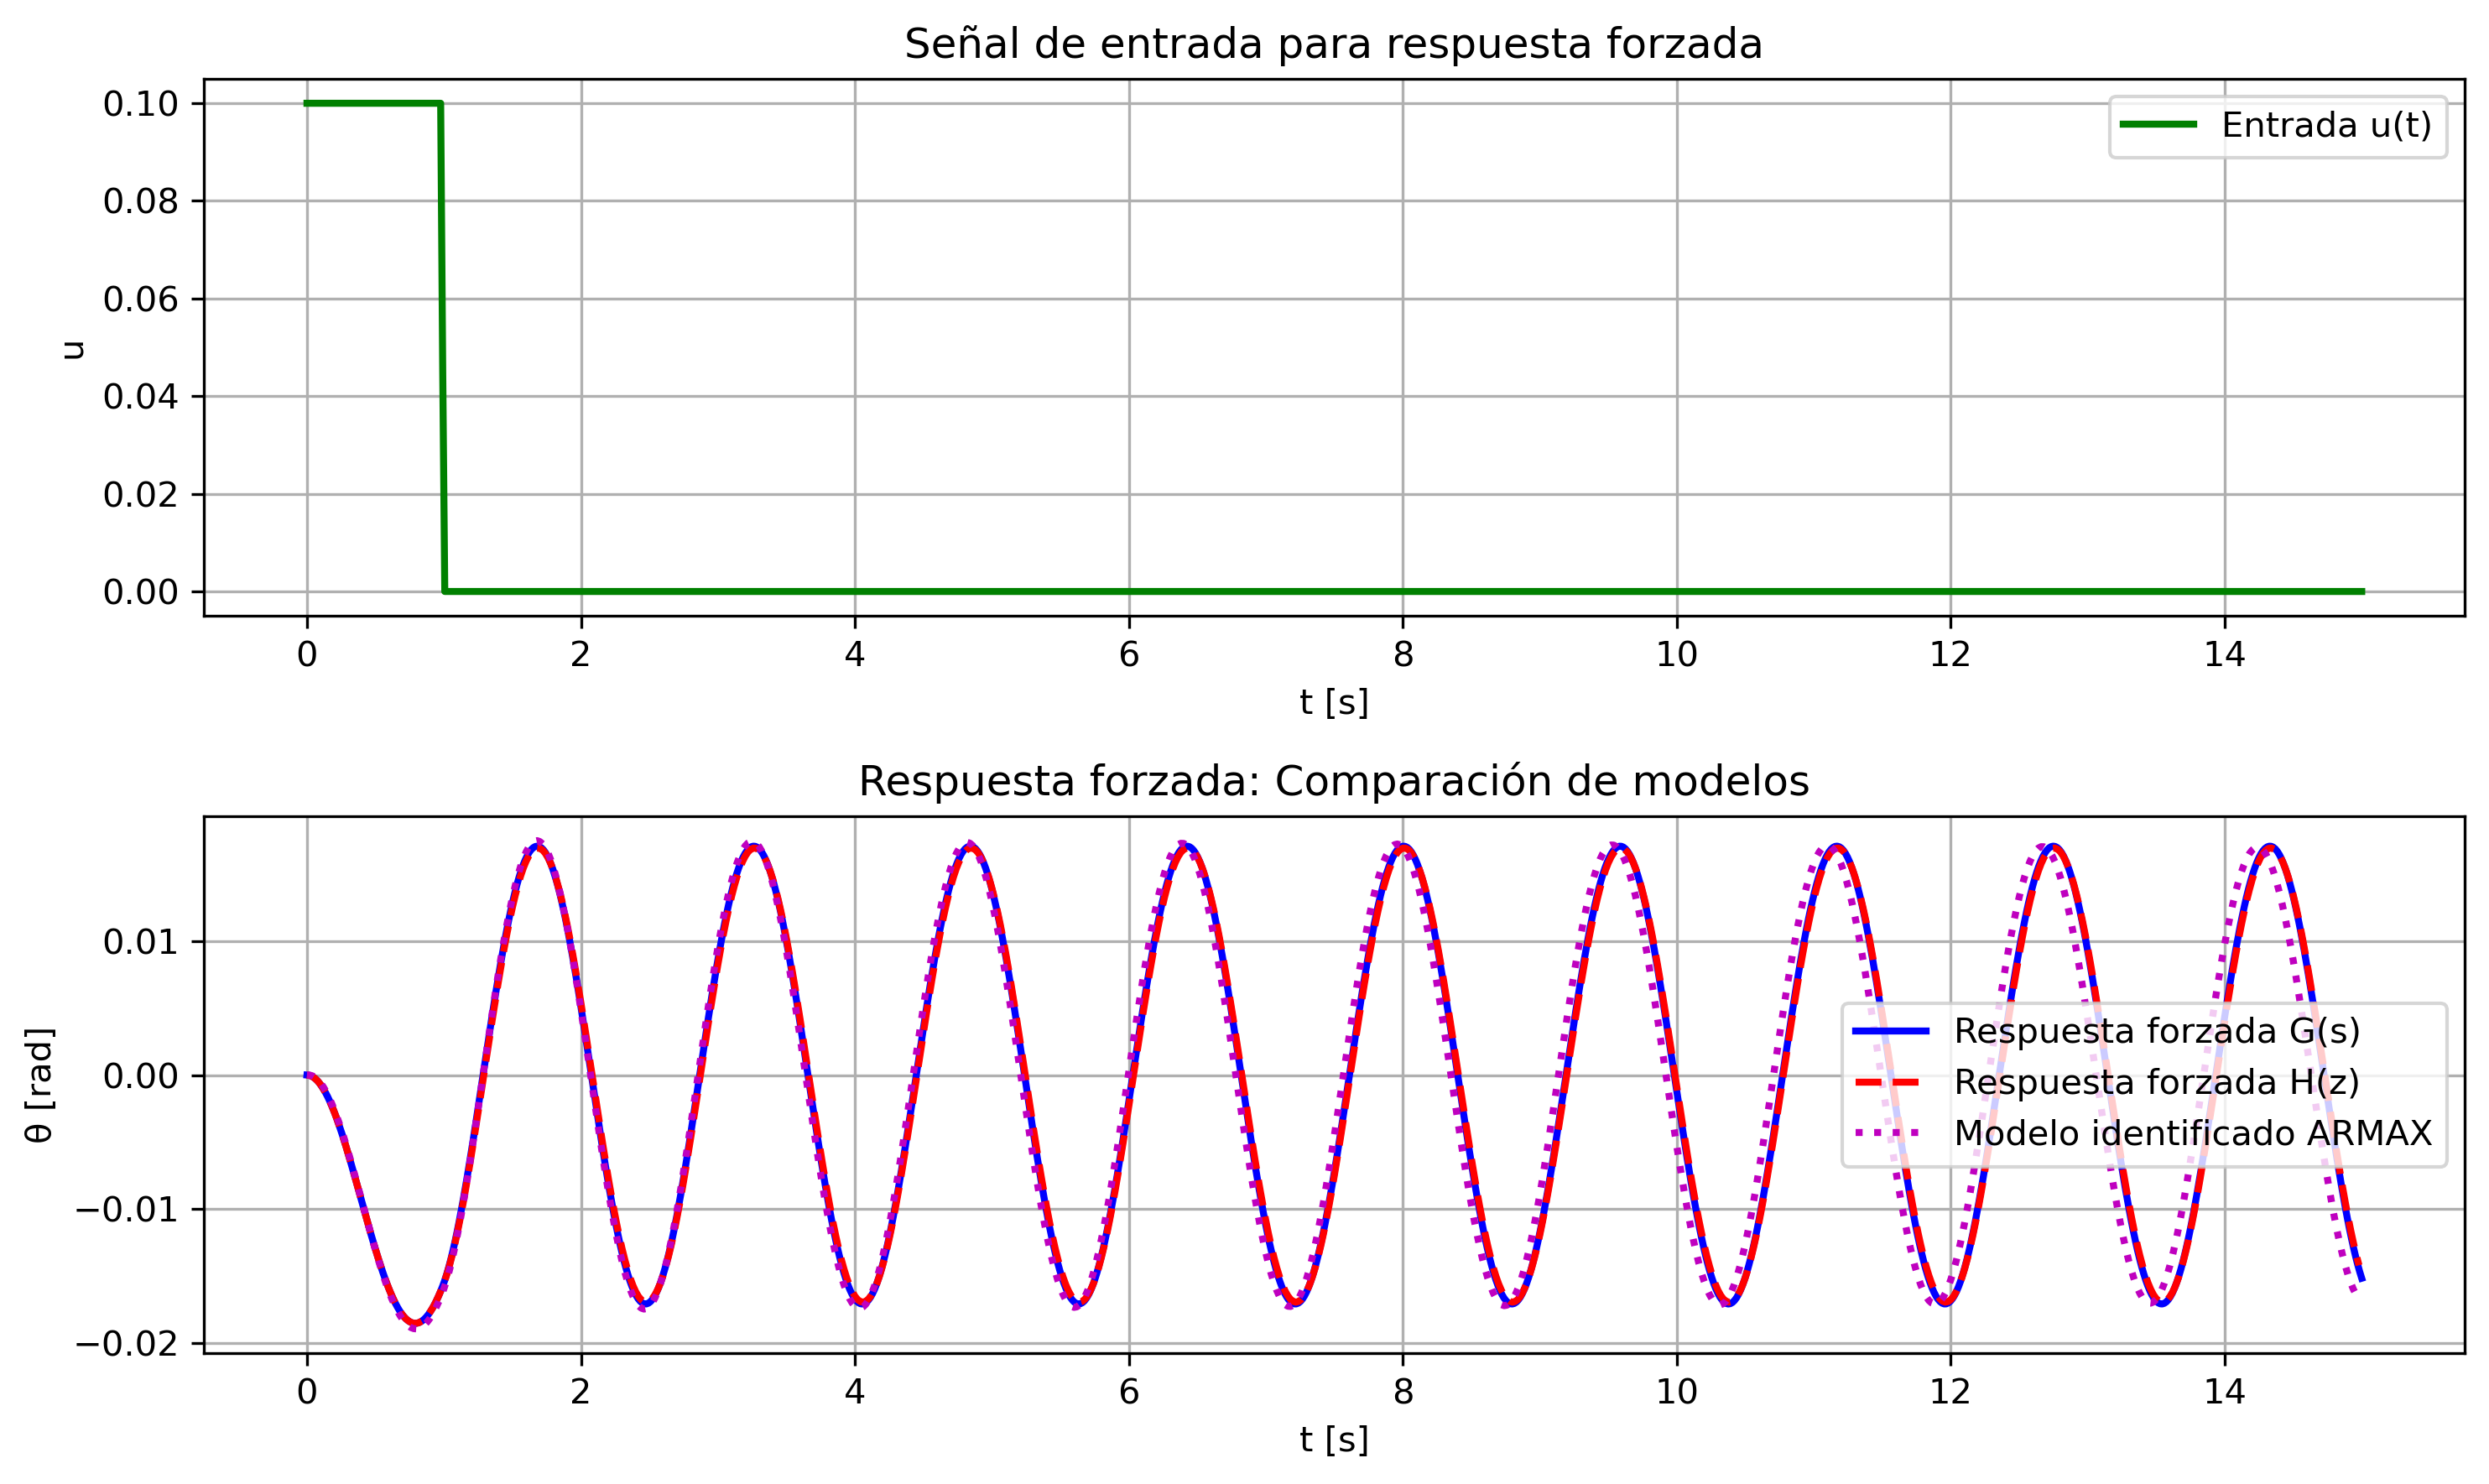
\includegraphics[width=\textwidth]{imagenes_identificacion/forced_response_comparison.png}
\caption{Comparación de respuesta forzada: Modelo continuo G(s), discreto H(z), e identificado ARMAX}
\label{fig:forced_response}
\end{figure}

\subsection{Análisis de Validación}

\begin{itemize}
\item \textbf{G(s) continuo:} Respuesta teórica exacta (referencia)
\item \textbf{H(z) discreto:} Discretización ZOH del sistema continuo
\item \textbf{ARMAX identificado:} Modelo experimental - excelente concordancia
\end{itemize}

La superposición casi perfecta entre los modelos teóricos y el identificado confirma el éxito de la identificación.

\section{Conclusiones}

\subsection{Principales Logros}

\subsubsection{Éxito Total de la Metodología}
- Identificación precisa de dinámica del sistema (error < 0.01\%)
- Modelo estable y físicamente consistente
- Validación estadística completa exitosa
- Simulación sin divergencia numérica

\subsubsection{Comparación con Enfoques Alternativos}
- Modelo ARMAX simplificado supera ampliamente a modelos ARX tradicionales
- Eliminación de coeficientes problemáticos mejora calidad global
- Enfoque parsimonioso resulta superior

\subsection{Contribuciones Metodológicas}

\subsubsection{Lecciones para Identificación de Sistemas}
\begin{enumerate}
\item \textbf{Diseño experimental apropiado:} Usar condiciones estables para identificación
\item \textbf{Selección de modelo:} Preferir modelos parsimoniosos sobre completos
\item \textbf{Validación estadística rigurosa:} Esencial para verificar calidad real
\item \textbf{Compromisos inteligentes:} Eliminar parámetros difíciles mejora resultados
\end{enumerate}

\subsubsection{Valor de la Validación Estadística}
- RMSE engañoso: El modelo ARMAX tiene RMSE bajo pero parámetros correctos
- Tests estadísticos revelan calidad real del modelo
- Validación estadística es condición necesaria y suficiente

\subsection{Conclusión Final}

Este trabajo demuestra que la \textbf{identificación exitosa} requiere:
\begin{itemize}
\item Entendimiento físico profundo del sistema
\item Metodología apropiada (ARMAX simplificado)
\item Diseño experimental cuidadoso
\item Validación estadística rigurosa desde el inicio
\end{itemize}

Sin estos elementos, incluso con técnicas avanzadas, la identificación está condenada al fracaso. Este trabajo sirve como \textbf{ejemplo de buenas prácticas} en identificación de sistemas, contrastando fuertemente con el fracaso documentado en el Trabajo Práctico 2.

\subsection{Nota sobre Implementación}

Los códigos fuente y gráficos generados automáticamente están disponibles en los directorios \code{identificacion\_pendulo.py} e \code{imagenes\_identificacion/}. La implementación utiliza Python con librerías científicas estándar (NumPy, SciPy, Matplotlib, Control).

\end{document}
